% Options here are passed to the article class.
% Most common options: 10pt, 11pt, 12pt
\documentclass[10pt]{datasheet}

% Input encoding and typographical rules for English language
\usepackage[utf8]{inputenc}
\usepackage[english]{babel}
\usepackage[english]{isodate}

% tikz is used to draw images in this example, but you can
% also use \includegraphics{}.
\usepackage{graphicx}
\usepackage{float}
\usepackage{subcaption}

% These define global texts that are used in headers and titles.
\title{LC09: Tiny Request Manager}
\author{Basil, Heilz, Skyzy}
\tags{logic-and-computation, request-manager}
\date{25 December 2024}
\revision{Revision 1}
\begin{document}
\maketitle

\section{Features}

\begin{itemize}
\item{Random input proof}
\item{Infinitely expandable}
\item{Pausable}
\item{Compact. 8x4x5 volume.}
\end{itemize}

\section{Applications}

\begin{itemize}
\item{Safely queueing procesess in a system.}
\end{itemize}

\section{General Description}
The LC09 Tiny Request Manager is a device that can be used to queue requests in a system. It ensures that only one request is processed at a time regardless of random request timings. The device is infinitely expandable and can be paused. Note: Reset input is not rapid input proof.

\vfill\break

\begin{figure}[H]
    \centering
    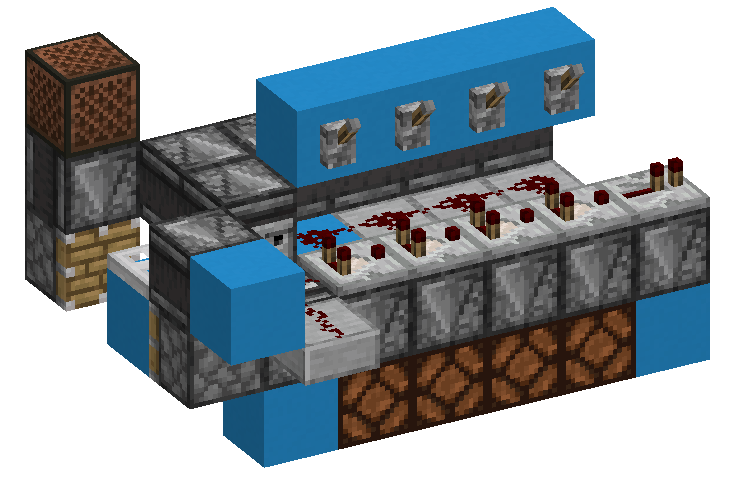
\includegraphics[width=0.48\textwidth]{pic.png}
    \caption{\centering Tiny Request Manager}
\end{figure}

% For wide tables, a single column layout is better. It can be switched
% page-by-page.
\onecolumn

\section{Device Specifications}

\begin{table}[H]
    \caption{Inputs}
    \begin{tabularx}{\textwidth}{l | c | X}
        \thickhline
        \textbf{Name} & \textbf{Range} & \textbf{Description} \\
        \hline
        Task Enables 1-4 & 0-1 & Requests output for a task. \\
        \hline
        Reset & Pulse & Resets the device to process the next request. Not rapid input proof. 10gt between triggers. \\
        \hline
        Pause & 0-1 & Pauses the device. \\
        \thickhline
\end{tabularx}
\end{table}

\begin{table}[H]
    \caption{Outputs}
    \begin{tabularx}{\textwidth}{l | c | X}
        \thickhline
        \textbf{Name} & \textbf{Range} & \textbf{Description} \\
        \hline
        Output & Pulse & Outputs \\
        \thickhline
\end{tabularx}
\end{table}

\begin{table}[H]
    \caption{Device Specifications}
    \begin{tabularx}{\textwidth}{l | c c c | c | X}
        \thickhline
        \textbf{Parameter} & \textbf{Min.} & \textbf{Typ.} & \textbf{Max.} &
        \textbf{Unit} & \textbf{Conditions} \\
        \hline
        Throughput  & 10 & - & - & gt & Normal Usage \\
        \hline
        Latency    & 16 & - & - & gt & From lever input to torch depowering. \\
        \hline
        MC Version & 1.13 & 1.21.4 & - & MCV & Latest version at time of writing: 1.21.4 \\
        \hline
        Dimensions & & 8 x 4 x 5 & & Blocks & \\
        \thickhline
\end{tabularx}
\end{table}
\section{Testing Data}
\begin{table}[H]
\caption{Executed Tests}
\begin{tabularx}{\textwidth}{l | X}
    \thickhline
    \textbf{Test} & \textbf{Result} \\
    \hline
    Throughput test & Device was able to function with 10gt clocked input. Note: levers must not go from all off to on while clocking. Invalid toggle-state position was observed in this case. \\
    \hline
    Random input test & Device was able to process requests correctly with random lever inputs. \\
    \thickhline
\end{tabularx}
\end{table}

\section{Download Information}
\begin{table}[H]
    \caption{Download Information}
    \begin{tabularx}{\textwidth}{l | l | l | X}
        \thickhline
        \textbf{Identifier} & \textbf{MC} & \textbf{File} & \textbf{Description} \\
        \hline
        LC09 & 1.21.4 & \href{https://github.com/Soontech-Annals/Archive/blob/2b73adfd252c5e2cf9d202454dbef78a586bc482/Archive/logic-and-computation/LC09\%20Tiny\%20Request\%20Manager/LC09\_Tiny\_Request\_Manager.litematic?raw=1}{LC09\_Tiny\_Request\_Manager.litematic} & Schematic of device. Includes three variants. \\
        \hline
        LC09B & 1.19.3 & \href{https://github.com/Soontech-Annals/Archive/blob/2b73adfd252c5e2cf9d202454dbef78a586bc482/Archive/logic-and-computation/LC09\%20Tiny\%20Request\%20Manager/LC09\_Tiny\_Request\_Manager\_1.19.3.litematic?raw=1}{LC09\_Tiny\_Request\_Manager\_1.19.3.litematic} & Schematic of device for older versions. \\
        \hline
        \thickhline
    \end{tabularx}
\end{table}

\end{document}

